\chapter{System Design}
\label{ch:design}

This chapter describes the incubator as it was built. Every component and the reason it was chosen is summarised in Appendix~\ref{app:selection-summary}, with the full option-by-option comparison and prices in Appendix~\ref{app:component-selection} and the bill of materials in Appendix~\ref{app:bom}.

%*********************************************************************
\section{System Overview}
\label{sec:system-overview}
%*********************************************************************

The incubator is a printed enclosure that holds a 96-well plate on the microscope stage at 37\,\textdegree{}C, near saturation, with 5\% CO\textsubscript{2}. Figure~\ref{fig:block-diagram} shows how the parts fit together.

\begin{figure}[htbp]
    \centering
    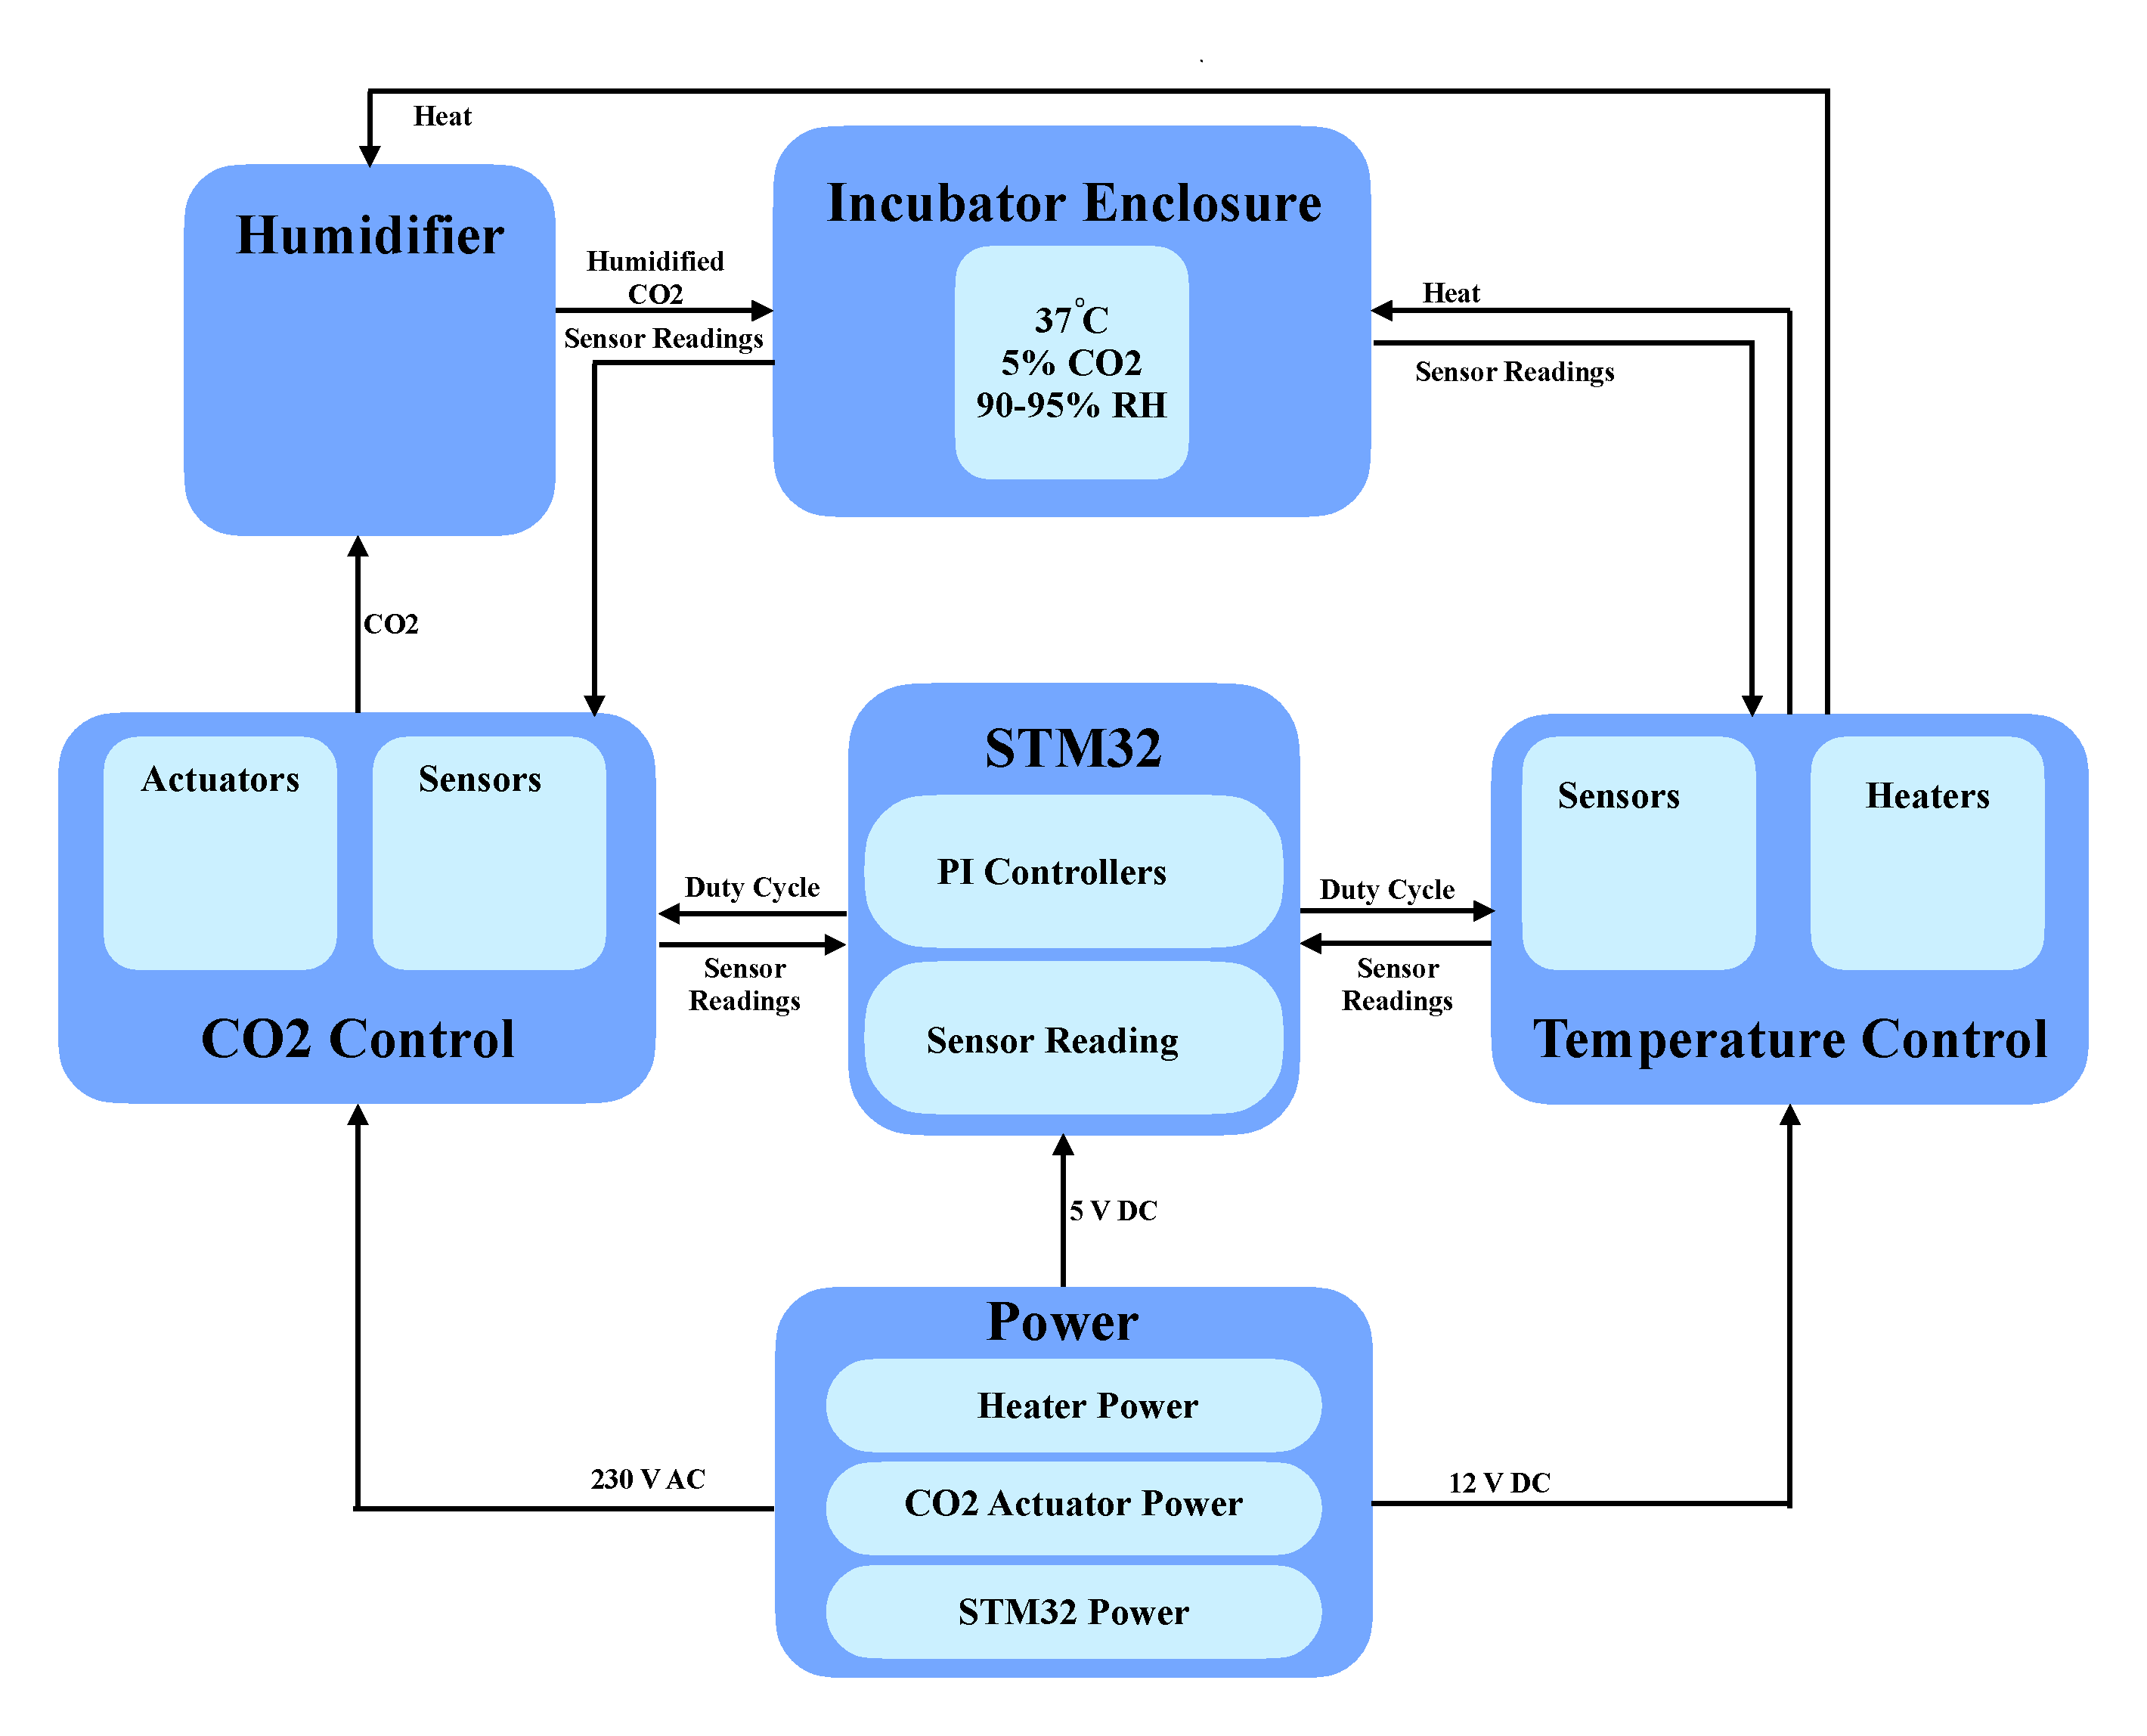
\includegraphics[width=0.62\textwidth]{figs/ch4/System Diagram.pdf}
    \caption[System architecture]{\textbf{System architecture.} Three loops close around one plant. The STM32 reads every sensor and sets a duty cycle for each actuator. CO\textsubscript{2} passes through a water-filled humidifier before entering the enclosure, so one gas line carries both CO\textsubscript{2} and water vapour. Humidity is measured but not controlled. The heat path to the humidifier was planned but not built (Section~\ref{sec:co2-design}).}
    \label{fig:block-diagram}
\end{figure}

The enclosure is the plant: the setpoints apply to it and everything else exists to hold them there. One STM32 runs the three PI loops designed in Chapter~\ref{ch:theory}, reading every sensor and setting a duty cycle for each actuator. Temperature is controlled through two heated zones with the same loop structure: film heaters on the walls set the air temperature, and an indium tin oxide (ITO) coated glass lid is both the optical window and a heating element. CO\textsubscript{2} reaches the chamber through a humidifier bottle, so one gas line carries both the gas and the water vapour. Humidity is measured but not controlled, so Chapter~\ref{ch:theory} treats it only as a constraint on the glass setpoint, and Chapter~\ref{ch:co2humidity} shows why this gas path alone cannot hold the chamber near saturation. Four thermistors and one PT1000 are read, and where each sat during testing is given in Section~\ref{sec:sysid-approach}.

%*********************************************************************
\section{Incubator Enclosure}
\label{sec:enclosure}
%*********************************************************************

\begin{figure}[H]
    \centering
    \begin{subfigure}[b]{0.30\textwidth}
        \centering
        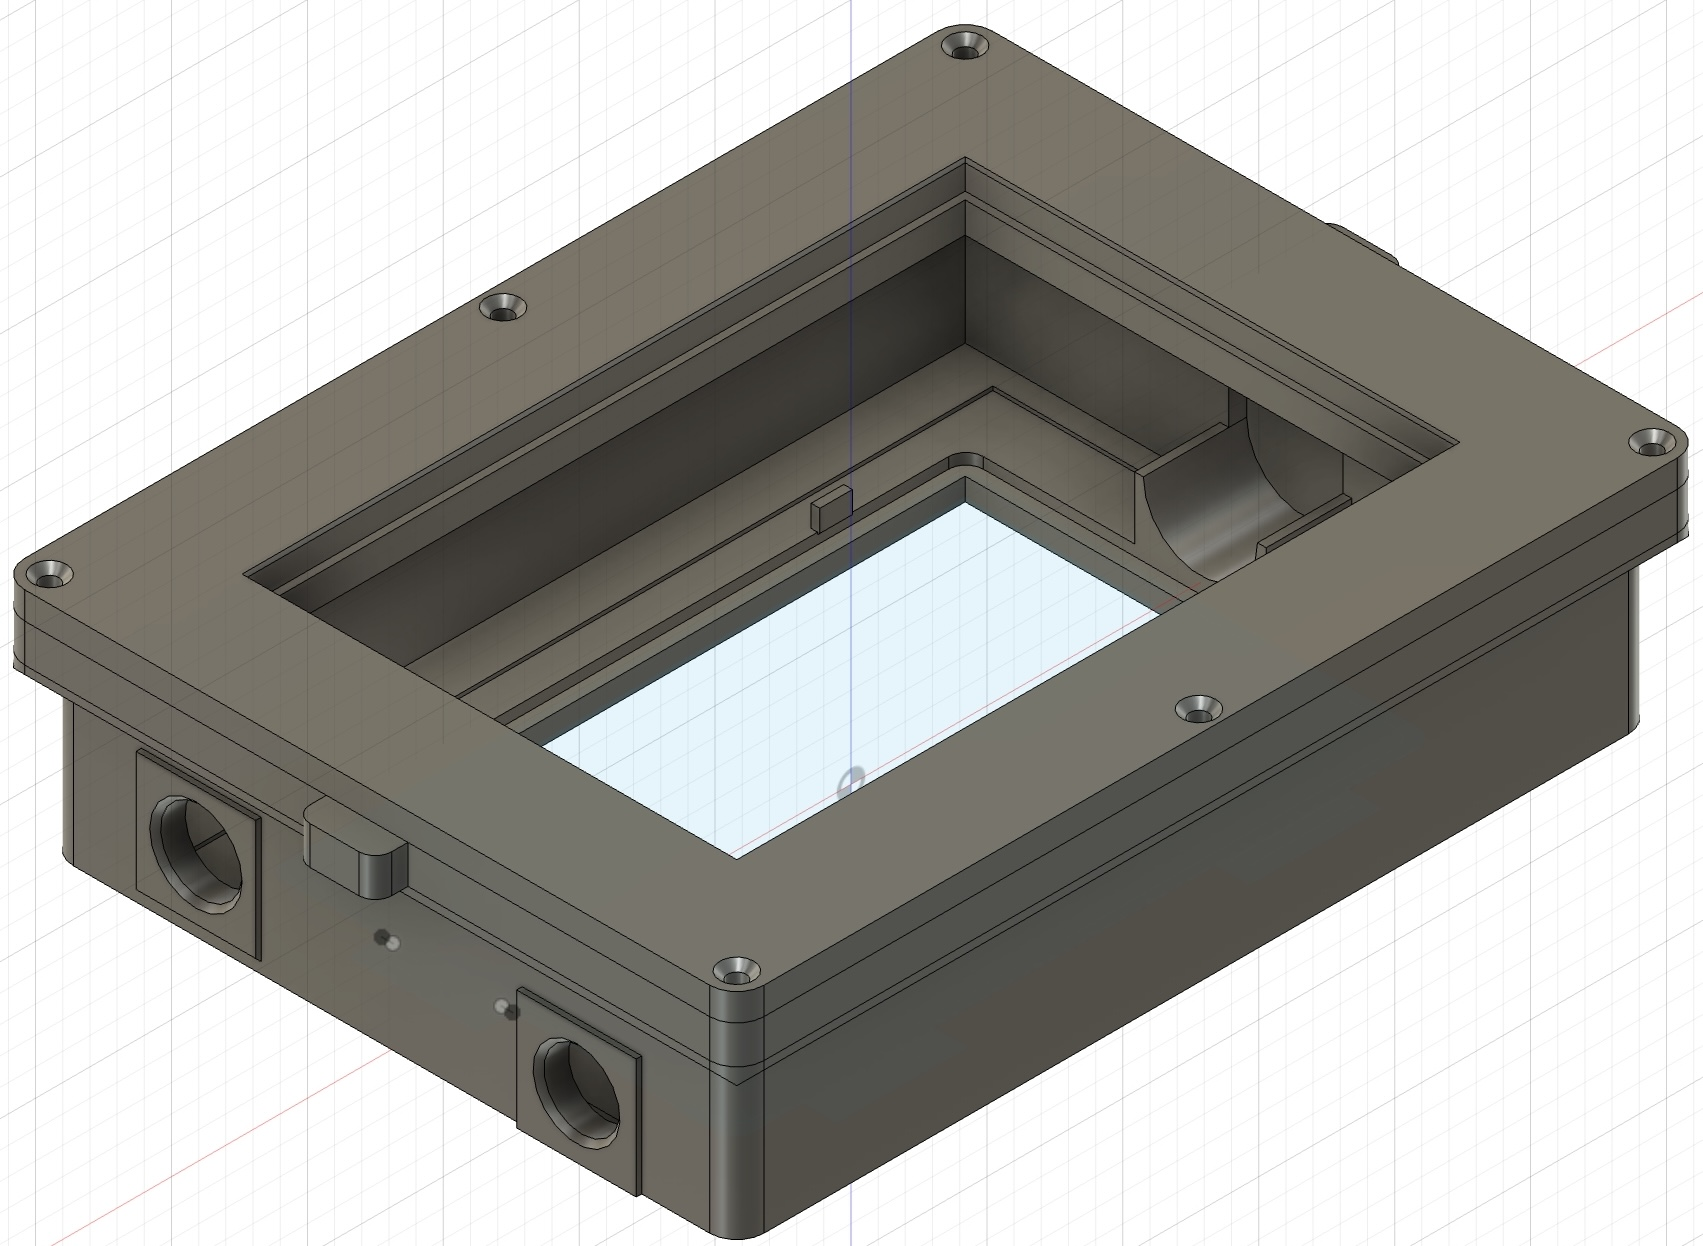
\includegraphics[width=\linewidth]{figs/ch4/incubator_isometric.jpg}
        \caption{}
        \label{fig:cad-iso}
    \end{subfigure}\hfill
    \begin{subfigure}[b]{0.30\textwidth}
        \centering
        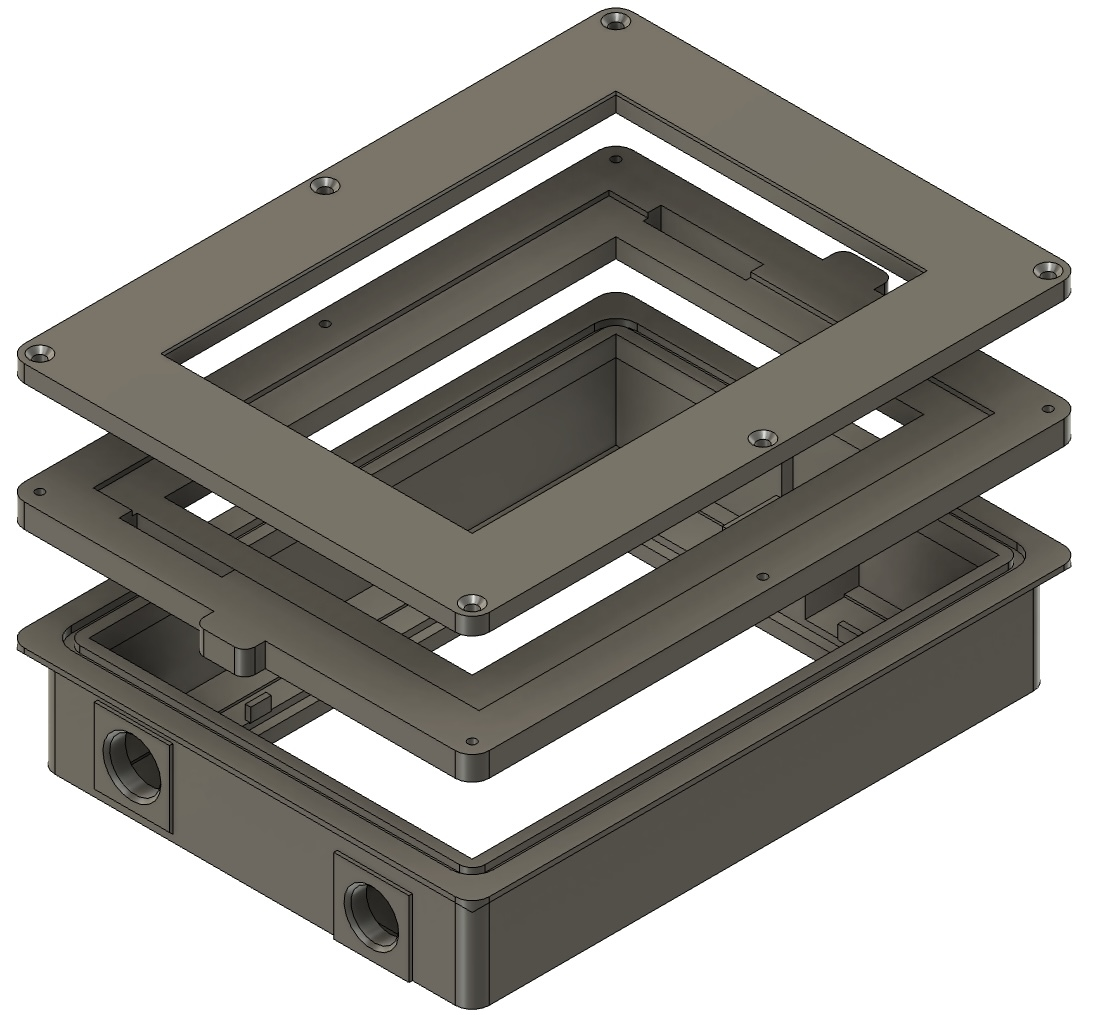
\includegraphics[width=\linewidth]{figs/ch4/incubator_exploded.jpg}
        \caption{}
        \label{fig:cad-exploded}
    \end{subfigure}\hfill
    \begin{subfigure}[b]{0.30\textwidth}
        \centering
        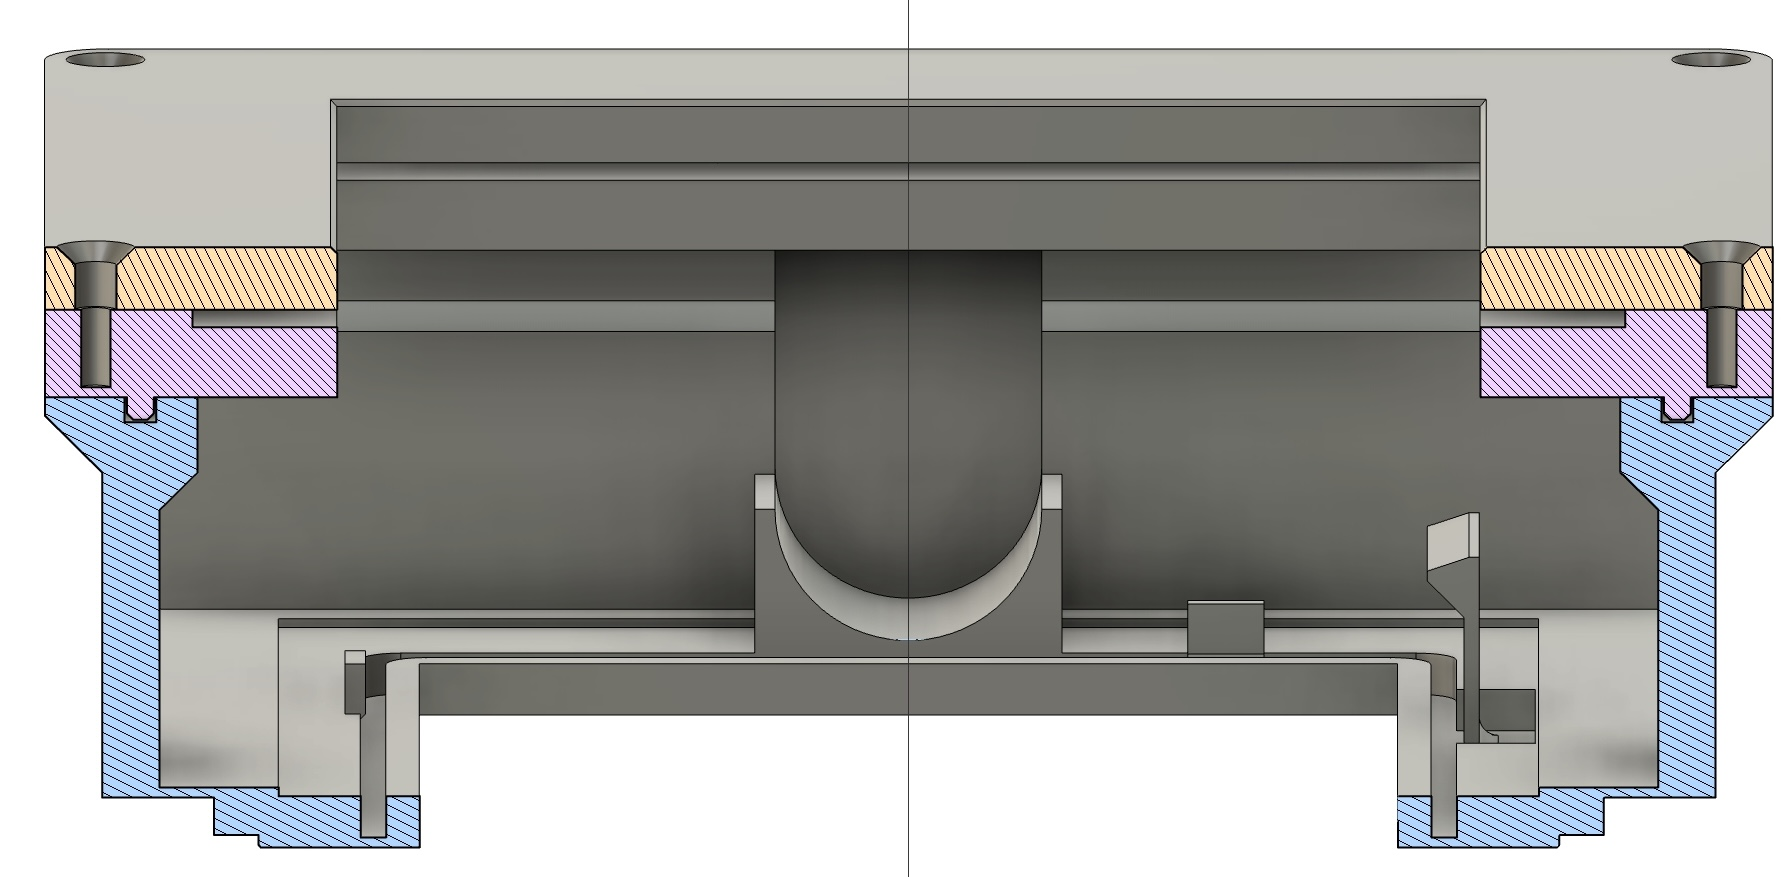
\includegraphics[width=\linewidth]{figs/ch4/incubator_section.jpg}
        \caption{}
        \label{fig:cad-section}
    \end{subfigure}
    \caption[Enclosure construction]{\textbf{Enclosure construction.} (a) The assembly closed. (b) The three printed parts: base, lid frame and bezel. (c) Section through the centre, showing the stepped plate seat, one of the clips, the CO\textsubscript{2} sensor seat and the lid rib sitting in its groove.}
    \label{fig:cad-assembly}
\end{figure}

\begin{table}[H]
    \centering
    \caption[Enclosure dimensions]{\textbf{Enclosure dimensions.} Origin: \textbf{M} measured on the microscope, \textbf{S} set by the plate or the glass supplier, \textbf{C} chosen, \textbf{D} follows from the others.}
    \label{tab:dims}
    \footnotesize
    \setlength{\tabcolsep}{4pt}
    \renewcommand{\arraystretch}{1.1}
    \begin{tabular}{@{}>{\raggedright\arraybackslash}p{3.5cm}>{\raggedright\arraybackslash}p{3.1cm}c@{\hspace{6mm}}>{\raggedright\arraybackslash}p{3.5cm}>{\raggedright\arraybackslash}p{3.1cm}c@{}}
        \toprule
        \textbf{Dimension} & \textbf{Value} & & \textbf{Dimension} & \textbf{Value} & \\
        \midrule
        Recess in the stage insert & 160 $\times$ 110\,mm, 3\,mm deep & M & Thickness of floor under the plate & 0.8\,mm & C \\
        Hole through the stage & 153 $\times$ 103\,mm, through a 1\,mm lip & M & Imaging hole in the floor & 119 $\times$ 77\,mm & C \\
        96-well plate, outside & 127.76 $\times$ 85.48\,mm & S & Hole for bulkhead connector & 14\,mm & C \\
        Area the 96 wells cover & 106 $\times$ 70\,mm & S & Hole for cable gland & 15\,mm & C \\
        ITO glass sheet & 150 $\times$ 112 $\times$ 1.1\,mm & S & Plate clip, each & 20 $\times$ 1.2\,mm, 16.3\,mm long & C \\
        Chamber inside & 160 $\times$ 118\,mm, 26\,mm deep & C & Base sits into the stage by & 4\,mm & D \\
        Chamber wall thickness & 4.5\,mm & C & Gap from top of plate to glass & 21.9\,mm & D \\
        \bottomrule
    \end{tabular}
\end{table}

The first consideration was the microscope. The incubator has to sit in the K-frame insert of an open-frame inverted stage, which was measured in person along with the base of an existing stage-top incubator that already fits it. Those measurements set the outside of the base, and the dimensions referred to below are listed in Table~\ref{tab:dims}. The underside is stepped to match the stage: the wider step sits in the shallow recess around the opening, and the narrower step drops through the opening itself with 0.3\,mm clearance on each side (Figure~\ref{fig:cad-section}). Nothing reaches more than 4\,mm below the top of the stage. Figure~\ref{fig:cad-assembly} shows the result. Everything else is built inward from there, as three parts printed in polyethylene terephthalate glycol (PETG): the base, a lid frame and a bezel.

\textbf{Holding the plate.} The plate needs a fixed place to sit, so the floor has a stepped recess shaped to it, with the plate rim landing on a ledge to give the same seated height every time. The floor under that ledge is the dimension that matters most, because it sets how high the sample sits above the stage, and the higher the sample sits the more of the objective's working distance is used up before the light reaches it. So the floor needs to be as thin as the printer nozzle allows. For the first iteration 0.8\,mm was chosen, two layers of a 0.4\,mm nozzle; anything thinner risks gaps and a floor that will not carry the plate. The opening in the floor is bigger than the well field, so the enclosure does not block the light path.

The recess supports the plate but does not hold it still, so three thin clips sit along the inside walls and press the plate against fixed faces on the other side (Figure~\ref{fig:cad-section}). They were made thin on purpose. A printed part is not as strong as solid PETG, because the layers do not bond as well, and how much weaker depends on the printer and the settings, none of which was known before the first print. Thin clips risk snapping, thick clips risk the plate not pushing past them at all, and for a first build the second is the worse problem.

\textbf{Sensors and connections.} The CO\textsubscript{2} sensor sits in a curved seat printed into the wall. Two holes go through the wall, one for the bulkhead connector and one for the cable gland (Figure~\ref{fig:cad-iso}). Both seal properly against the wall and both can be unscrewed and replaced easily, which is the standard way of passing cables and tubes through walls.

\textbf{Lid and seal.} The lid has two jobs, holding the ITO glass flat and getting the wires that power the glass out of the chamber, and one part cannot do both, so the lid is two (Figure~\ref{fig:cad-exploded}). The frame has a shallow pocket that the glass drops into and the bezel clamps it from above, stopping against the frame rather than against the glass so that tightening a screw presses on plastic and not on a 1.1\,mm sheet. The wires run out through slots in the frame beside the glass. The lid simply drops onto the base, with a raised rib sitting in a matching groove in the base rim and nothing clamping the two together. Screws would seal better and a second version should use them, but during testing the lid needs to come on and off many times. The chamber is therefore not perfectly sealed. This is accounted for: the CO\textsubscript{2} model in Chapter~\ref{ch:theory} includes the leak, and the leak is what sets the time constant. It is small enough to cost gas without making the chamber unstable \citep{talebipour_facilitating_2024}.

\textbf{Printing and limitations.} The model was checked for the problems that could appear after printing. No part has a closed pocket that could trap moisture or support material, no wall is thinner than 0.8\,mm apart from the deliberate floor, and overhangs are cut back to 45\,\textdegree{} so support is only needed on exposed outer faces. What the model cannot show is left to testing: the CO\textsubscript{2} sensor has no cover above it, so condensation landing on its window is a risk; the seal was never measured for how much it leaks; and nothing was printed and measured before the design was committed, so the accuracy of the thin sections and how well the clips hold up are only known once it is built. These are carried into Chapter~\ref{ch:commissioning}.

%*********************************************************************
\section{Temperature Control}
\label{sec:temperature-design}
%*********************************************************************

\begin{figure}[htbp]
    \centering
    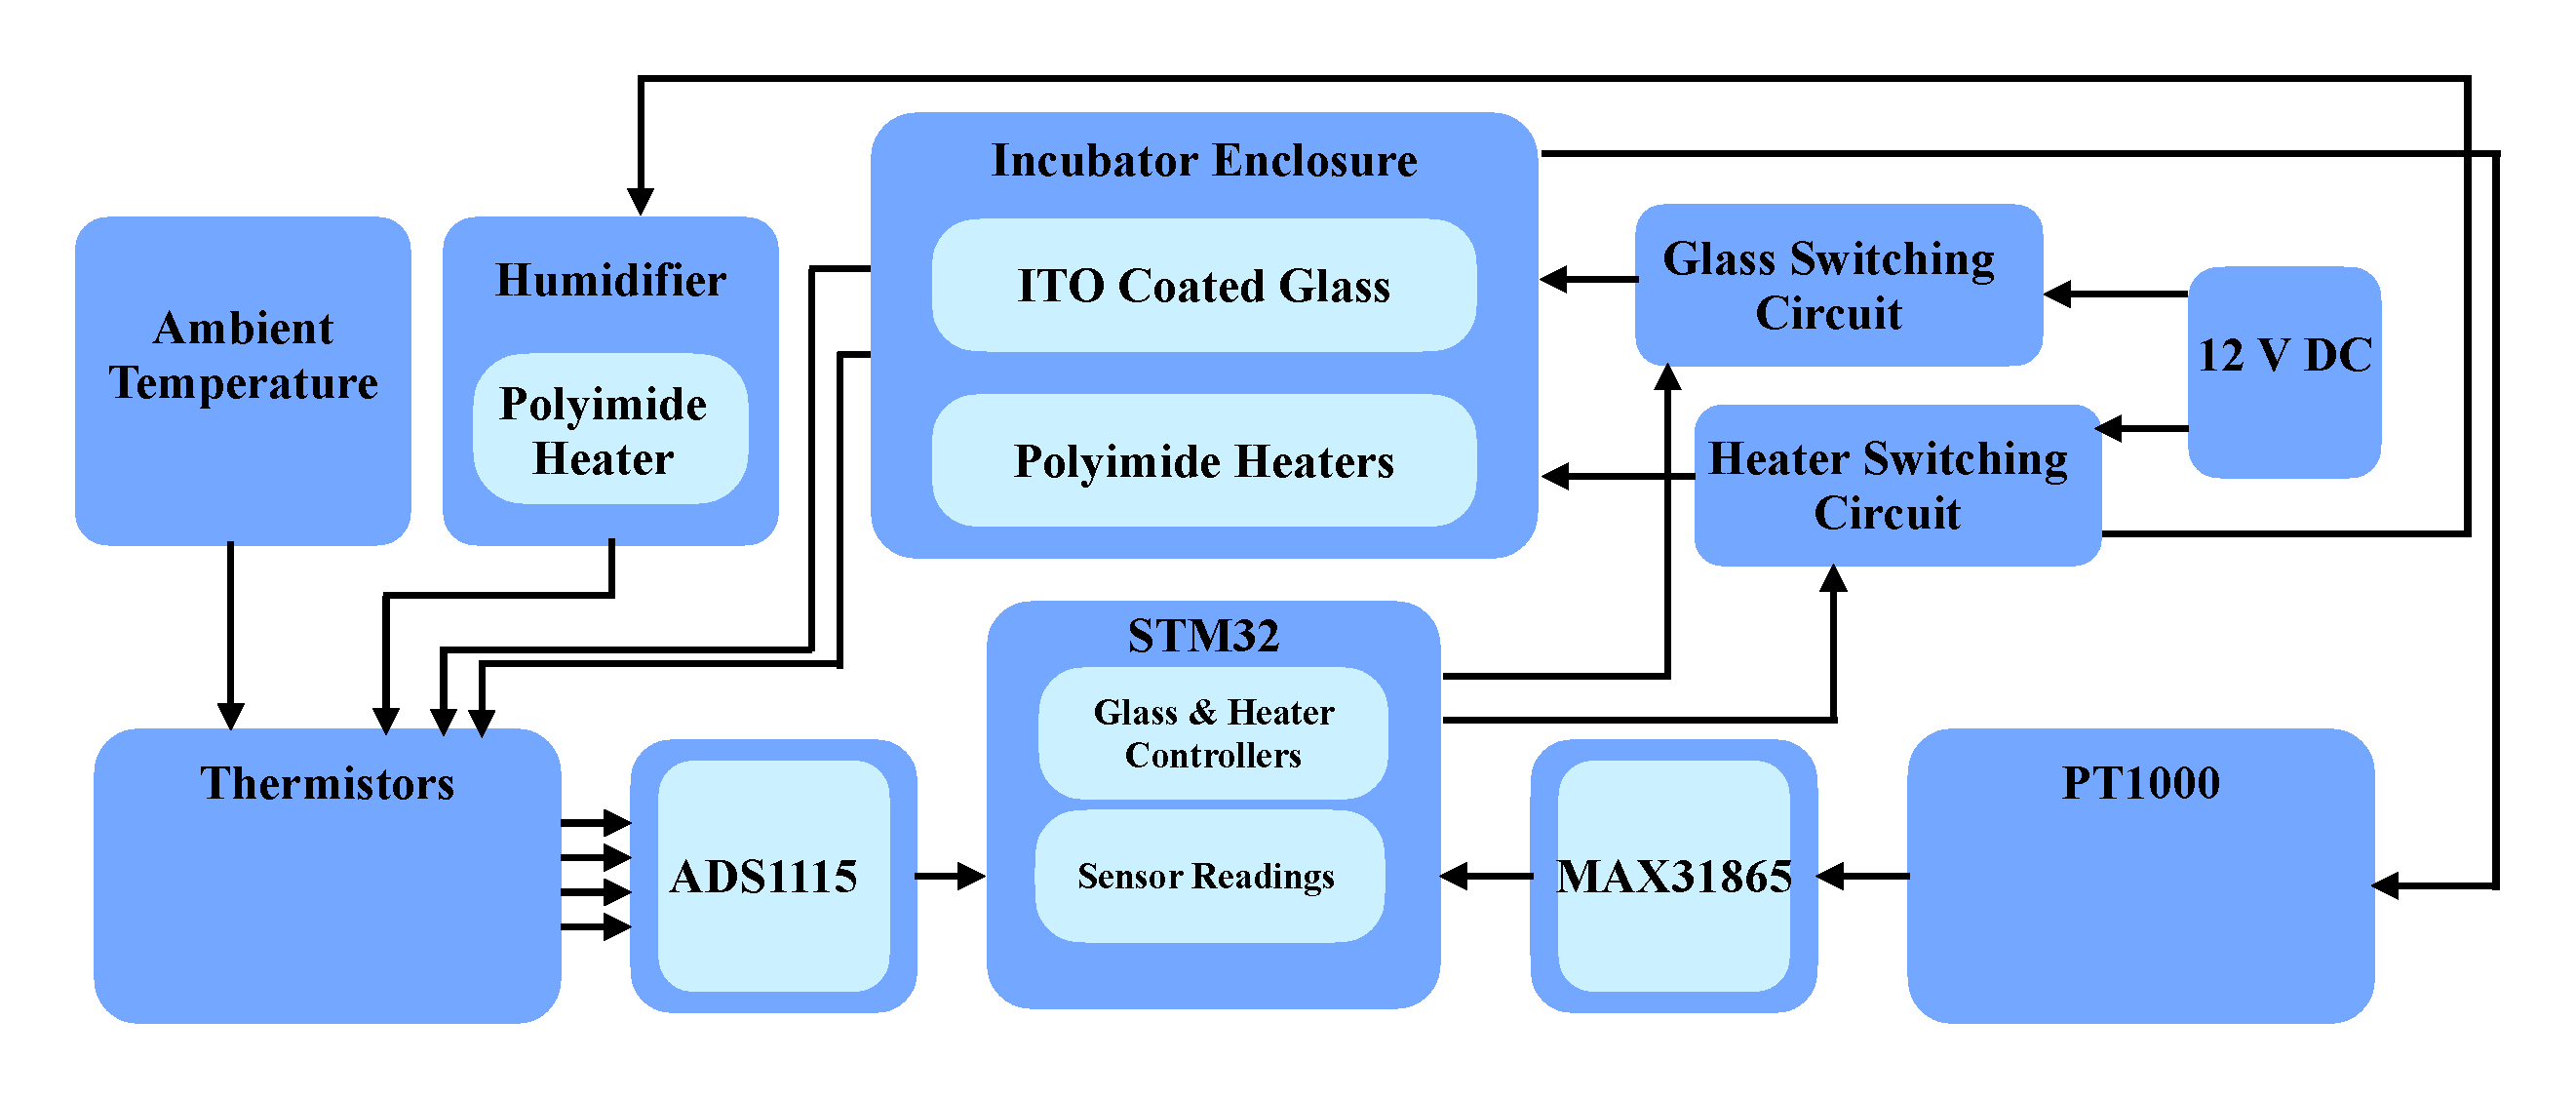
\includegraphics[width=0.62\textwidth]{figs/ch4/Temperature Control.pdf}
    \caption[Temperature control subsystem]{\textbf{Temperature control subsystem.} Four thermistors are read through an ADS1115 and the PT1000 through a MAX31865. The PT1000 is the calibration reference for the thermistors and, during bench testing, the control sensor for the chamber air. The STM32 drives each heater through a transistor pair that switches the 12\,V rail. The humidifier heater shown was planned but not built.}
    \label{fig:temp-diagram}
\end{figure}

Figure~\ref{fig:temp-diagram} shows the subsystem: the heated zones, the measurement channels, the two converters that read them, and the switching circuits between the STM32 and the heaters. R1 and R2 set the tolerance at $\pm$0.3\,\textdegree{}C, so the sensors need a resolution well below 0.3\,\textdegree{}C for the requirement to be testable.

\textbf{Chamber heaters.} The reviewed incubators all heat with flexible resistive elements stuck to a surface (Section~\ref{subsec:existing-temperature}). Cartridge heaters were ruled out first, since the heated tip is small so the heat comes from a point rather than a surface, and there is nowhere convenient to mount one inside a 26\,mm chamber. Silicone mats spread heat well, but the smallest size sold locally was larger than the chamber wall. Polyimide film heaters suit the job: they heat over an area, come in strips that match the wall dimensions, and have an adhesive backing. The 12\,V range was chosen because it had the sizes that fit and is sold in a 20-pack, which leaves room to change how many pads are used, move them, or add a zone later without reordering. Chapter~\ref{ch:theory} modelled three pads at 12\,W, 36\,W in total, because the model was built before the enclosure was printed. The build uses two pads on opposite walls, for the reasons given in Section~\ref{sec:sysid-approach}, and the lower heater power is carried into the model identified from the built chamber in Chapter~\ref{ch:thermalID}. This also set the supply: with the heaters at 12\,V, a single 12\,V rail runs the rest of the system.

\textbf{Heated glass lid.} A heated transparent lid is standard across the reviewed systems. ITO glass was chosen because the coating is a transparent resistive layer, so current through it heats the whole surface evenly while transmitting over 80\% of visible light \citep{konshen_ito_2026}, and Ragazzini heats a chamber this way directly \citep{ragazzini_fabrication_2019}. Sheet resistance had to be specified at order time because it sets the available power: at 12\,V the panel gives about 2\,W at 50\,$\Omega$/sq and 21\,W at 5\,$\Omega$/sq. A 5 to 10\,$\Omega$/sq coating was specified, giving 10.7 to 21.5\,W. The same calculation ruled out the cheaper ITO-coated PET film, made only in a 50\,$\Omega$/sq grade, which was bought as a fallback before the glass was quoted and is not used in the built system.

The known limitation is optical. Section~\ref{subsec:existing-temperature} records that Ragazzini cut a hole in the ITO layer and fitted a plain coverslip, because even a high-transmittance coating cuts enough light to matter for phase contrast. Transmission through this lid was not measured, since the focus of this project is the control system and stage time was not available for optical testing, so it is left to future work (Chapter~\ref{ch:furtherwork}). The lid is removable, so a plain uncoated sheet can be fitted and the two compared whenever that test is done.

\textbf{No heating from below.} This is a deliberate departure from the comparison in Section~\ref{subsec:existing-comparison}. The path below the plate is the one the objective images through, so a heated layer there would add a second coated surface to the optics. An objective heater was also omitted, since the laboratory already has one and Section~\ref{subsec:existing-drift} notes a poorly regulated one can worsen focal drift rather than reduce it. Spare pads are held back in case either is needed. Section~\ref{sec:cl-test3} returns to this: heating the plate from below is what finally brings a well to 37\,\textdegree{}C, and the optical question raised here is still open.

\textbf{Temperature sensing.} Resistance temperature detectors (RTDs) are the most accurate option in principle, so they were the starting point against R1. Not all of them reach it: under IEC 60751 a Class A element is about $\pm$0.22\,\textdegree{}C at 37\,\textdegree{}C and a Class B about $\pm$0.49\,\textdegree{}C \citep{iec_60751_2008}, so only Class A or better qualifies, and a probe that does not state its class cannot be trusted to. Wiring matters as much: lead resistance adds straight into a 2-wire reading, costing 0.5 to 1\,\textdegree{}C on a PT100 with a metre of cable, but only about 0.1\,\textdegree{}C on a PT1000, which is the same element built to ten times the resistance. What decided it was size, since probes with a stated class are bulky and four will not fit inside a 26\,mm chamber alongside a well plate.

So the RTD is the reference. One Class A PT1000 gives a ground truth, and the distributed measuring is done by thermistors small enough to fit, a format several of the reviewed systems use. During bench testing the PT1000 also served as the control sensor for the chamber air, since it is the most accurate and steadiest channel and the system was being modelled and tuned. It is not intended for that role in use on the microscope stage, where the probe is too large to sit in the chamber beside the plate, and a calibrated thermistor would take its place. The same part sits in all four positions, including the reservoir and the room where $\pm$0.5\,\textdegree{}C would do, because one part number means one calibration against the PT1000 rather than a curve per type. The PT1000 is read through a MAX31865, which is built for RTDs and drives and measures the element itself \citep{maxim_max31865_2015}. The thermistors would take four analogue pins, so they go to an ADS1115 analogue-to-digital converter (ADC) over the inter-integrated circuit (I\textsuperscript{2}C) bus instead, which costs two: sixteen bits leave the thermistor's nonlinearity as the limit rather than the resolution, and the programmable gain matches the input range to the voltage swing around 37\,\textdegree{}C \citep{ti_ads1115_2018}.

\textbf{Heater control.} The STM32 cannot drive the heaters directly, since its pins supply a few milliamps and the heaters draw amps, so each heater is switched by a pair of transistors instead. The STM32 sends its PWM signal to a PN2222A, the PN2222A drives a TIP31C, and the TIP31C carries the heater current. Both parts were already in the laboratory. A MOSFET would be the better choice, because the TIP31C drops over a volt while it is on and turns a few watts into heat, where a logic-level MOSFET would drop a fraction of that. This is a change for a second iteration rather than a problem for the prototype.

%*********************************************************************
\section{CO\textsubscript{2} Control and Humidity}
\label{sec:co2-design}
%*********************************************************************

This section covers the CO\textsubscript{2} Control and Humidifier blocks of Figure~\ref{fig:block-diagram}, taken together because they sit on one gas line. Figure~\ref{fig:co2-subsystem} follows that line in full, from the cylinder through to the enclosure, and the subsections below take it in the same order. R4 sets the tolerance at $\pm$0.3 percentage points, so the sensing needs a resolution well below that at the setpoint and a range that extends above it, since a controller designed to avoid overshoot cannot be judged by a sensor that saturates there.

\begin{figure}[htbp]
    \centering
    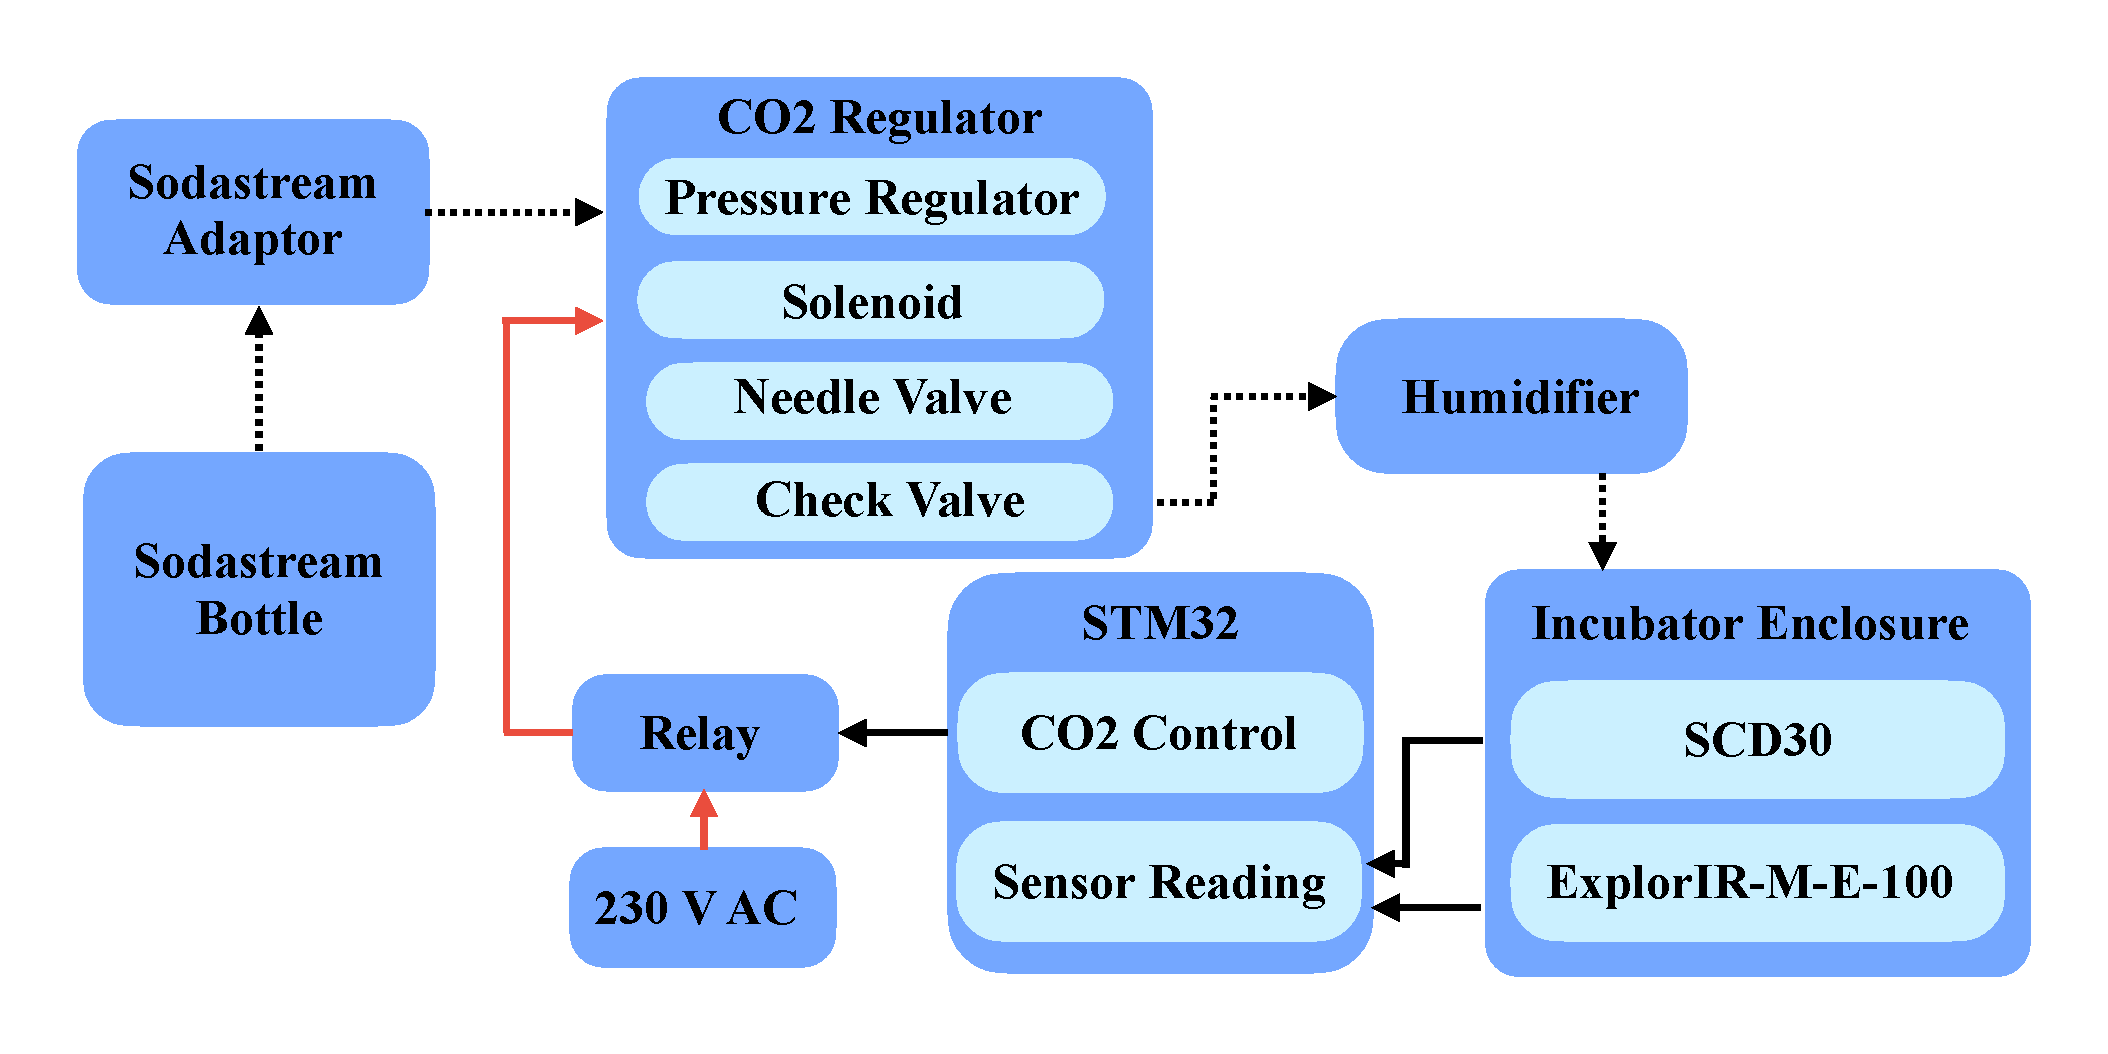
\includegraphics[width=0.62\textwidth]{figs/ch4/CO2 Control.pdf}
    \caption[CO\textsubscript{2} control subsystem]{\textbf{CO\textsubscript{2} control subsystem.} Dotted lines carry CO\textsubscript{2}, the red line is the 230\,V mains and solid black lines are signals. Gas passes from the cylinder through the regulator assembly and bubbles through the humidifier, so one line carries both the CO\textsubscript{2} and the water vapour into the enclosure. The STM32 closes the loop on the two sensors by switching the mains solenoid through a relay.}
    \label{fig:co2-subsystem}
\end{figure}

\textbf{Regulation and valves.} Chapter~\ref{ch:review} selected a cylinder and solenoid over premixed gas blending, because it needs no laboratory gas line and reuses the same sensor-and-valve structure as the other loops. The gas path then needs four things: a regulator to drop cylinder pressure to a working pressure, a solenoid for the controller to act on, a needle valve to set the flow, and a check valve to stop humidifier water being drawn back into the line. These were first priced as separate pneumatic components. An aquarium CO\textsubscript{2} regulator sold as a single assembly does all four for roughly half the cost of the regulator and solenoid alone (Appendix~\ref{app:co2-valve-options}), and it was chosen for more than the price: separate parts have to be matched on thread and pressure rating, where an assembly sold as one unit is already matched, so there is less that can go wrong on arrival. The supplier is also local, so it could be collected in person and the fit confirmed with the vendor beforehand.

The one place supplier data could not be relied on was the cylinder connection. The listing said the regulator inlet was G5/8, which is not the G1/4 Type 30 standard used on South African cylinders. The supplier was contacted and confirmed that the regulator does fit South African cylinders, because the inlet is in fact Type 30 and the listing was wrong. Thread specifications from a product listing should be confirmed with the supplier before ordering any parts that depend on them.

\textbf{Gas supply.} Industrial cylinders were priced first, through Air Products, a local gas supplier that already has an account with UCT. They were rejected on access rather than price: a cylinder of that size has to be rented on a supplier account, which many laboratories do not hold, and it is heavy and difficult to transport. A SodaStream cylinder was chosen instead. It is food-grade CO\textsubscript{2}, sold and exchanged in ordinary retail shops, so anyone rebuilding this design can get gas without a supplier account, and it is small enough to carry, which suits an instrument meant to move between microscopes. The small volume helps during testing as well, since a 60\,L cylinder cannot put anywhere near as much CO\textsubscript{2} into the room as an industrial one if a fitting leaks or the solenoid is left open. Gas costs more per litre this way, which is the tradeoff accepted. A SodaStream cylinder does not use the Type 30 valve the regulator takes, so a cylinder adapter connects the two (Appendix~\ref{app:co2-valve-options}).

The solenoid is mains-powered and switched through a relay module that isolates the logic side, which is the red mains path in Figure~\ref{fig:co2-subsystem}. One tube size, 6\,mm outside diameter and 4\,mm inner, is used throughout: it is what the regulator assembly and the bulkhead fittings both take, so any section of the line can be remade without an adapter.

\textbf{Humidifier.} Section~\ref{subsec:existing-humidity} showed that systems with external humidification bubble the gas through a water reservoir on its way into the chamber. The same arrangement was built from a sealed container with two holes in the lid. A cable gland in each hole clamps the tube where it passes through, which holds the seal better than glue would. The CO\textsubscript{2} tube runs down into the water so the gas bubbles up through it, and the second tube stops above the water so the gas leaves from the air above. Keeping the reservoir outside the enclosure avoids the capacity problem in Section~\ref{subsec:existing-humidity}, where a small internal tank runs dry within hours. Humidity is not controlled: the SCD30 measures it and nothing acts on it. Heating the reservoir with a spare film pad was considered, but not built. The gas only flows while the solenoid is open, so the humidifier wets only the CO\textsubscript{2} stream, and Section~\ref{sec:humidity} shows that this stream is far too small a share of the air entering the chamber to hold it near saturation.

\textbf{Gas sensing.} Section~\ref{subsec:existing-co2} showed that every CO\textsubscript{2}-controlled system uses an NDIR sensor, so the only thing left to decide was the range. A 5\% setpoint is 50\,000\,ppm, and the obvious sensors are the ones sold to read up to exactly that. The problem with a sensor only reaching 5\% is that it returns the same value for anything at or above 5\%, so any overshoot is not measured, and the controller could then not be tested against the one behaviour it is meant to avoid. The search therefore moved to sensors reading up to 100\%. The chosen ExplorIR-M-E-100 is accurate to $\pm$(300\,ppm $+$ 5\% of reading), or about $\pm$0.28\% CO\textsubscript{2} at setpoint \citep{gss_explorir_2021}, which Section~\ref{subsec:existing-accuracy} puts in the same band as the commercial systems at their looser end, and just inside the $\pm$0.3 percentage points of R4.

Humidity is measured by an SCD30 on the same I\textsuperscript{2}C bus as the thermistor converter, so it uses no extra pins \citep{sensirion_scd30_2020}. It also reports CO\textsubscript{2}, and using it for both would have saved the cost of the ExplorIR, but its 40\,000\,ppm ceiling sits below the setpoint so it cannot be the control sensor. That channel is still logged below 4\% as a cross-check, since two independent readings make a sensor fault easier to spot. Both sensors sit inside the chamber, rated to 95\% RH non-condensing, and automatic baseline correction is disabled on both, since it assumes regular exposure to fresh air at roughly 400\,ppm, which a sealed incubator never sees.

%*********************************************************************
\section{Power and Embedded Platform}
\label{sec:power-design}
%*********************************************************************

Everything except the solenoid runs from a single 12\,V rail, since the heaters are 12\,V parts and the ITO power calculation assumes 12\,V. Capacity was sized against the heaters, which dominate, before the number of wall pads was settled: three wall pads at 12\,W plus the glass at up to 21.5\,W is about 58\,W. A 120\,W adapter was chosen so that every heated zone can run at full power together during warm-up with room for an extra zone, which later covered the heated base added in Chapter~\ref{ch:ClosedLoop}. A buck converter rated well above the logic-side draw steps 12\,V down to 5\,V for the microcontroller and sensors. The solenoid is the one component outside this rail, running on mains through its relay.

An STM32 platform was a requirement from the outset, so the question was which part, and peripheral count decided it. The design needs three PWM outputs, a digital output for the CO\textsubscript{2} relay, a universal asynchronous receiver-transmitter (UART) for the CO\textsubscript{2} sensor, I\textsuperscript{2}C for the thermistor converter and humidity sensor, a serial peripheral interface (SPI) for the RTD converter, and a second UART for logging. The STM32L476RG provides three I\textsuperscript{2}C interfaces, five USARTs, three SPI interfaces and sixteen timers \citep{st_stm32l476_2019}, so all are available at once; on a smaller part two peripherals often share pins, which only becomes apparent during integration when both are needed together. Its floating point unit matters more than its clock speed, since three integral terms accumulate over runs lasting a day or more. A Nucleo-64 board was used rather than a bare chip or custom PCB for its on-board programmer and header access, since this prototype is rewired repeatedly during characterisation.

%*********************************************************************
\section{Cost}
\label{sec:bom}
%*********************************************************************

The bill of materials in Appendix~\ref{app:bom} totals R\,13\,527, including import duties on the glass, and excluding the Nucleo board, printed filament, fasteners and wiring. This satisfies R10: an order of magnitude below the commercial systems costed in Section~\ref{subsec:existing-comparison} and in the same band as the DIY builds. Two items dominate, the CO\textsubscript{2} sensor at 25\% and the ITO glass with duties at another 25\%. Both would be bought again, since nothing cheaper reads above 50\,000\,ppm and nothing cheaper heats a transparent lid evenly.

%*********************************************************************
% End of System Design
%*********************************************************************